\documentclass[12pt, twoside]{article}
\usepackage[letterpaper, margin=1in, head=30pt, headsep=0.1in]{geometry}
\usepackage[english]{babel}
\usepackage[utf8]{inputenc}
\usepackage{amsmath}
\usepackage{amsfonts}
\usepackage{amssymb}
\usepackage{tikz}
\usetikzlibrary{quotes, angles}

\usepackage{graphicx}
\usepackage{enumitem}
\usepackage{multicol}

%\usepackage{pgfplots}
%\pgfplotsset{width=10cm,compat=1.9}
%\usepgfplotslibrary{statistics}
%\usepackage{pgfplotstable}
%\usepackage{tkz-fct}
%\usepackage{venndiagram}

\usepackage{fancyhdr}
\pagestyle{fancy}
\fancyhf{}
\renewcommand{\headrulewidth}{0pt} % disable the underline of the header
\raggedbottom
\newif\ifmeta
\metatrue %print standards and topics tags

\title{Math AI Worksheet Generator and Formative Assessment System}
\author{Chris Huson}
\date{October 2020}

%\fancyhead[RE]{\thepage}
%\fancyhead[RO]{\thepage \\ Name: \hspace{3cm}}
%\fancyhead[L]{BECA / Dr. Huson / 10th Grade Geometry\\* 7 June 2019}
%
%\begin{document}
%\subsubsection*{13.7 Homework: Cross sections, distance applications}
%\fancyhead[L]{BECA / Dr. Huson / Geometry 03-Volume+angle-bisectors\\* pset ID: 34}

\begin{document}

\subsubsection*{2.6 Classwork Angle terminology}
\begin{enumerate}

\item Definition: \emph{Opposite rays} are collinear rays with a common end point.
\begin{enumerate}
  \item $\overrightarrow{BA}$ and $\overrightarrow{BC}$ are opposite rays
  \hspace{2cm}
    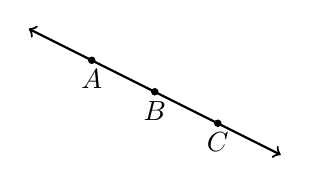
\begin{tikzpicture}[scale=.8]
      \draw  [<->, thick] (0,2)--(4,0);
      \draw [fill] (1,1.5) circle [radius=0.05] node[below]{$A$};
      \draw [fill] (2,1) circle [radius=0.05] node[below]{$B$};
      \draw [fill] (3,0.5) circle [radius=0.05] node[below]{$C$};
    \end{tikzpicture}
  \item These rays do not make a straight line.
  \hspace{1cm}
    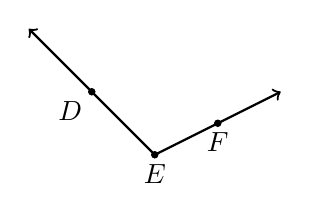
\begin{tikzpicture}[scale=.8]
      \draw  [<->, thick] (0,2)--(2,0)--(4,1);
      \draw [fill] (1,1) circle [radius=0.05] node[below left]{$D$};
      \draw [fill] (2,0) circle [radius=0.05] node[below]{$E$};
      \draw [fill] (3,0.5) circle [radius=0.05] node[below]{$F$};
    \end{tikzpicture}
  \item The rays $\overrightarrow{GH}$ and $\overrightarrow{HG}$ do not share a common end point.
    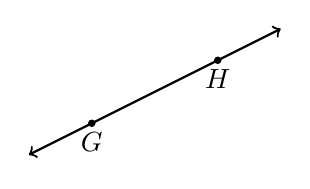
\begin{tikzpicture}[scale=.8]
      \draw  [<->, thick] (0,-2)--(4,0);
      \draw [fill] (1,-1.5) circle [radius=0.05] node[below]{$G$};
      \draw [fill] (3,-0.5) circle [radius=0.05] node[below]{$H$};
      %\draw [fill] (3,0.5) circle [radius=0.05] node[below]{$C$};
    \end{tikzpicture}
  \end{enumerate}
\newpage

\item Type your answers. Use the less than key (``$<$'') to represent an angle, followed by three letters. \vspace{0.25cm}
  \begin{enumerate}
    \item Name a right angle: \rule{4cm}{0.15mm} \bigskip
    \item Name the ray opposite to $\overrightarrow{OE}$: \rule{4cm}{0.15mm} \bigskip
    \item What is the measure of $\angle AOC$?  \rule{4cm}{0.15mm} \bigskip
    \item Name the angle vertical to $\angle AOB$: \rule{4cm}{0.15mm}
  \end{enumerate}
  \begin{center}
  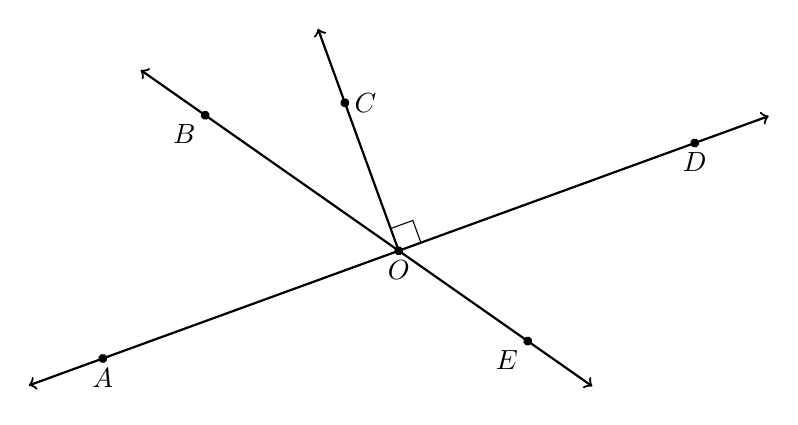
\begin{tikzpicture}[scale=1, rotate=20]
    \draw [<->, thick] (-55:3)--(0,0)--(125:4);
    \draw [<->, thick] (-5,0)--(5,0);
    \draw [->, thick] (0,0)--(0,3);
    \draw (0,0)++(0.3,0)--++(0,0.3)--+(-0.3,0);
    %\draw [fill] (-1,2.5) circle [radius=0.05] node[left ]{$B$};
    \draw [fill] (125:3) circle [radius=0.05] node[below left]{$B$};
    \draw [fill] (-4,0) circle [radius=0.05] node[below]{$A$}; 
    \draw [fill] (0,0) circle [radius=0.05] node[below]{$O$};
    \draw [fill] (0,2) circle [radius=0.05] node[right]{$C$};
    \draw [fill] (4,0) circle [radius=0.05] node[below]{$D$};
    \draw [fill] (-55:2) circle [radius=0.05] node[below left]{$E$};
  \end{tikzpicture}
  \end{center}
  \newpage

  \item As shown below, two lines intersect making four angles: $\angle 1$, $\angle 2$, $\angle 3$, and $\angle 4$.
  
    \begin{multicols}{2}
      Given $m\angle 1 = 75^\circ$.  
      \begin{enumerate}
        \item Find $m\angle 3$ \vspace{2cm}
        \item Find $m\angle 2$ \vspace{2cm}
      \end{enumerate}
      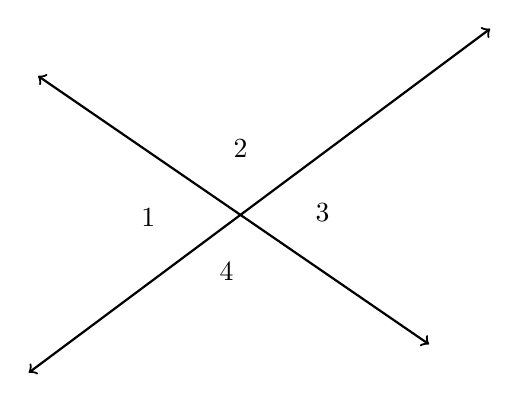
\begin{tikzpicture}[scale=0.7, rotate=20]
      \draw [<->, thick] (0,-1.5)--(10,1.5);
      \draw [<->, thick] (2,3.5)--(7,-3.5);
      \node at (3,.4){1};
      \node at (6,-.6){3};
      \node at (5,1){2};
      \node at (4,-1){4};
      %\draw [fill] (0,0) circle [radius=0.05] node[below]{$P$};
      %\draw [fill] (6,0) circle [radius=0.05] node[below]{$R$};
      %\draw [fill] (3,0) circle [radius=0.05] node[below]{$Q$};
    \end{tikzpicture}
    \end{multicols}

\newpage
\subsubsection*{Angle addition situations}

\item Apply the Angle Addition postulate. Write and equation to support your work.
  \begin{multicols}{2}
    Given $m\angle ABD = 80^\circ$ and \\[0.25cm] $m\angle DBC = 35^\circ$. \\[0.5cm]
    Find $m \angle ABC$. \\
    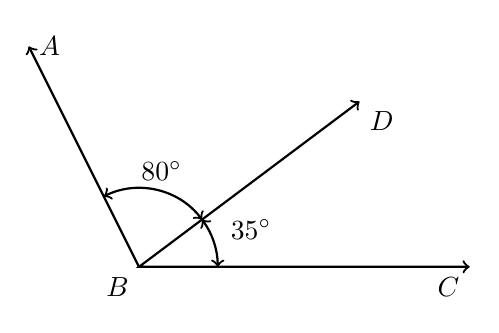
\begin{tikzpicture}[scale=1.4]
      \draw [<->, thick]
        (3,0) coordinate (a) node[below left] {$C$}
        -- (0,0) coordinate (b) node[below left] {$B$}
        -- (2,1.5) coordinate (c) node[below right] {$D$}
        pic["$35^\circ$", <->, draw=black, angle eccentricity=1.5, angle radius=1cm]
        {angle=a--b--c};
        \draw [<-, thick]
        (-1,2) coordinate (d) node[right] {$A$}
        -- (0,0) coordinate (e)
        pic["$80^\circ$", <->, draw=black, angle eccentricity=1.25, angle radius=1cm]
        {angle=c--e--d};
    \end{tikzpicture}
  \end{multicols}

  \newpage
  \item Given the angle measures and situation shown, write an equation and solve for $x$.
    \begin{multicols}{2}
      $m\angle ABD = 2x$ \\[0.25cm]
      $m\angle DBC = 50^\circ$ \\[0.25cm]
      $m \angle ABC = 110^\circ$ \\
      \begin{tikzpicture}[scale=2]
        \draw [<->, thick]
          (-20:2.5) coordinate (a) node[below left] {$C$}
          -- (0,0) coordinate (b) node[below left] {$B$}
          -- (30:3) coordinate (c) node[below right] {$D$}
          pic["$50^\circ$", <->, draw=black, angle eccentricity=1.5, angle radius=1cm]
          {angle=a--b--c};
          \draw [<-, thick]
          (80:2) coordinate (d) node[right] {$A$}
          -- (0,0) coordinate (e)
          pic["$2x$", <->, draw=black, angle eccentricity=1.5, angle radius=1cm]
          {angle=c--e--d};
      \end{tikzpicture}
    \end{multicols}

  \newpage
  \item The ray $\overrightarrow{BD}$ makes a $90^\circ$ angle with the line $\overleftrightarrow{ABC}$, and $m\angle DBE = x^\circ$, $m\angle EBC = 25^\circ$. \\[0.5cm] 
  Find $x$, writing and equation to support your work.
    \begin{flushright}
      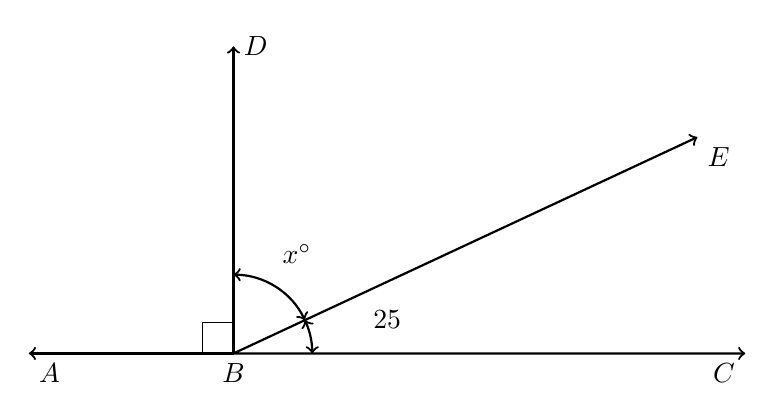
\begin{tikzpicture}[scale=1.3]
        \draw [<->, thick]
          (0:5) coordinate (a) node[below left] {$C$}
          -- (0,0) coordinate (b) node[below] {$B$}
          -- (25:5) coordinate (c) node[below right] {$E$}
          pic["$25$", <->, draw=black, angle eccentricity=2, angle radius=1cm]
          {angle=a--b--c};
          \draw [<-, thick]
          (90:3) coordinate (d) node[right] {$D$}
          -- (0,0) coordinate (e)
          pic["$x^\circ$", <->, draw=black, angle eccentricity=1.5, angle radius=1cm]
          {angle=c--e--d};
          \draw [->, thick] (0,0)--(-180:2) node[below right]{$A$};
          \draw (0,0)++(-0.3,0)--++(0,0.3)--+(0.3,0);
      \end{tikzpicture}
    \end{flushright}

  \newpage
  \item Two supplementary angles have measures $m\angle ABD = 5x$ and $m\angle DBC = 125^\circ$. \\[0.5cm] 
  Write an equation, then find $x$. \vspace{0.5cm}
    \begin{flushright}
      \begin{tikzpicture}[scale=1]
        \draw [<->, thick]
          (0:5) coordinate (a) node[below left] {$C$}
          -- (0,0) coordinate (b) node[below] {$B$}
          -- (125:3) coordinate (c) node[above right] {$D$}
          pic["$125^\circ$", <->, draw=black, angle eccentricity=1.5, angle radius=1cm]
          {angle=a--b--c};
          \draw [<-, thick]
          (180:4) coordinate (d) node[below] {$A$}
          -- (0,0) coordinate (e)
          pic["$5x$", <->, draw=black, angle eccentricity=1.5, angle radius=1cm]
          {angle=c--e--d};
          %\draw [->, thick] (0,0)--(-180:2) node[below right]{$A$};
          %\draw (0,0)++(-0.3,0)--++(0,0.3)--+(0.3,0);
      \end{tikzpicture}
    \end{flushright}
      
  \newpage
  \item Given the perpendicular situation shown, $\overrightarrow{BD} \perp \overleftrightarrow{ABC}$ and angle measures given. \\[0.5cm] 
  Find $x$. \vspace{0.5cm}
    \begin{multicols}{2}
      $m\angle DBE = 40^\circ$ \\[0.25cm]
      $m\angle EBC = 3x + 5^\circ$ \\[0.25cm]
      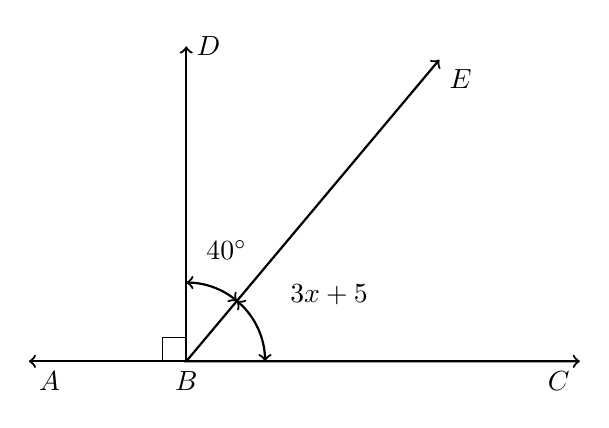
\begin{tikzpicture}[scale=1]
        \draw [<->, thick]
          (0:5) coordinate (a) node[below left] {$C$}
          -- (0,0) coordinate (b) node[below] {$B$}
          -- (50:5) coordinate (c) node[below right] {$E$}
          pic["$3x + 5$", <->, draw=black, angle eccentricity=2, angle radius=1cm]
          {angle=a--b--c};
          \draw [<-, thick]
          (90:4) coordinate (d) node[right] {$D$}
          -- (0,0) coordinate (e)
          pic["$40^\circ$", <->, draw=black, angle eccentricity=1.5, angle radius=1cm]
          {angle=c--e--d};
          \draw [->, thick] (0,0)--(-180:2) node[below right]{$A$};
          \draw (0,0)++(-0.3,0)--++(0,0.3)--+(0.3,0);
      \end{tikzpicture}
    \end{multicols}

  \newpage
  \item A linear pair have measures $m\angle ABD = 7x + 16^\circ$ and $m\angle DBC = 5x + 20^\circ$. \\[0.5cm] 
  Find $m\angle ABD$. \vspace{0.5cm}
    \begin{flushright}
      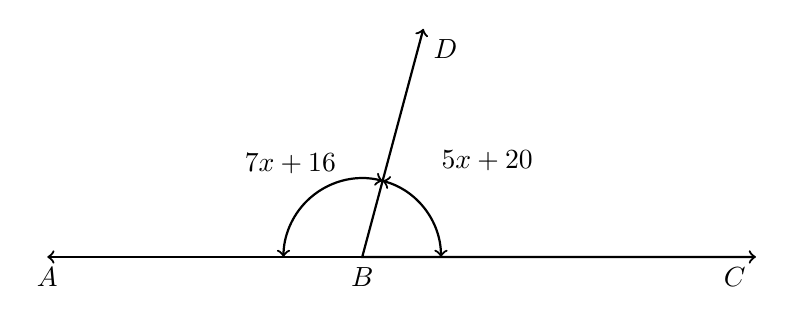
\begin{tikzpicture}[scale=1]
        \draw [<->, thick]
          (0:5) coordinate (a) node[below left] {$C$}
          -- (0,0) coordinate (b) node[below] {$B$}
          -- (75:3) coordinate (c) node[below right] {$D$}
          pic["$5x + 20$", <->, draw=black, angle eccentricity=2, angle radius=1cm]
          {angle=a--b--c};
          \draw [<-, thick]
          (180:4) coordinate (d) node[below] {$A$}
          -- (0,0) coordinate (e)
          pic["$7x + 16$", <->, draw=black, angle eccentricity=1.5, angle radius=1cm]
          {angle=c--e--d};
          %\draw [->, thick] (0,0)--(-180:2) node[below right]{$A$};
          %\draw (0,0)++(-0.3,0)--++(0,0.3)--+(0.3,0);
      \end{tikzpicture}
    \end{flushright}

\newpage
\item Given $\overline{DEFG}$, $DE=3 \frac{1}{4}$, $EF=6 \frac{1}{4}$, and $FG= 1 \frac{3}{4}$. (diagram not to scale)\\ [0.25cm]
  Find ${DG}$, expressed as a fraction, not a decimal.
  \begin{flushright}
      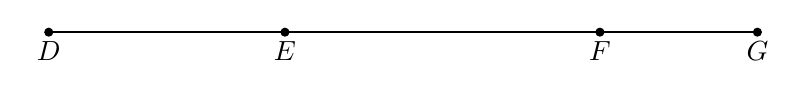
\begin{tikzpicture}
        \draw [-, thick] (0,0)--(9,0);
        \draw [fill] (0,0) circle [radius=0.05] node[below]{$D$};
        \draw [fill] (3,0) circle [radius=0.05] node[below]{$E$};
        \draw [fill] (7,0) circle [radius=0.05] node[below]{$F$};
        \draw [fill] (9,0) circle [radius=0.05] node[below]{$G$};
      \end{tikzpicture}
    \end{flushright}

\newpage
\item Given $P(-2.4)$ and $Q(1.8)$, as shown on the number line. \\[0.25cm]
  Find the length of the line segment $\overline{PQ}$. State an equation for full credit.
  \begin{center}
    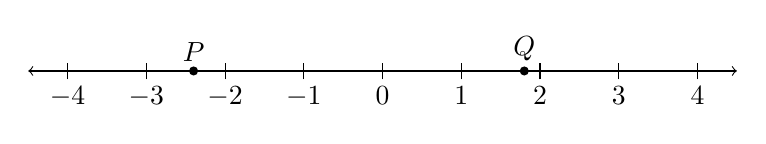
\begin{tikzpicture}
      \draw [<->] (-4.5,0)--(4.5,0);
      \draw [-, thick] (-2.4,0)--(1.8,0);
      \foreach \x in {-4,...,4} %2 leading for diff!=1
        \draw[shift={(\x,0)},color=black] (0pt,-3pt) -- (0pt,3pt) node[below=5pt]  {$\x$};
        \draw [fill] (-2.4,0) circle [radius=0.05] node[above] {$P$};
        \draw [fill] (1.8,0) circle [radius=0.05] node[above] {$Q$};
    \end{tikzpicture}
  \end{center}

\end{enumerate}
\end{document}